\documentclass[titlepage]{tufte-book}

\usepackage[runall=true]{pythontex}
\setpythontexworkingdir{<outputdir>}
\usepackage{environ}
\usepackage{morewrites}
\usepackage{amsthm}
\usepackage{amsmath}
\usepackage{amssymb}
\usepackage[pdftex]{graphicx}
\usepackage{epstopdf}
\usepackage{hyperref}
\usepackage{alltt}
\usepackage{listings}
\usepackage{array}
\usepackage{extarrows}
\usepackage{setspace}
\usepackage{tikz}
\usepackage{tikz-qtree}
\usetikzlibrary{calc}
\usetikzlibrary{positioning}
\usepackage{hyperref}
\usepackage{graphviz}
\usepackage{geometry}                % See geometry.pdf to learn the layout options. There are lots.
\usepackage{bashful}
\usepackage{microtype} % Improves character and word spacing
\usepackage{caption}

\usepackage{booktabs} % Better horizontal rules in tables

\setkeys{Gin}{width=\linewidth,totalheight=\textheight,keepaspectratio} % Improves figure scaling
\graphicspath{{figures/}}

\usepackage{fancyvrb} % Allows customization of verbatim environments
\fvset{fontsize=\normalsize} % The font size of all verbatim text can be changed here

\newcounter{problem}
\newcounter{total}
\newcommand{\step}[1]{{}
\vspace{4pt} \noindent {\bf \theproblem. }#1\addtocounter{problem}{1}}

\newcommand{\cut}[1]{}

\usepackage[tikz]{bclogo}
\usepackage{tikz}
\usetikzlibrary{calc}

\lstdefinestyle{BashInputStyle}{
  language=bash,
  basicstyle=\small\ttfamily,
  numberstyle=\tiny,
  showstringspaces=false,
  numbersep=3pt,
  otherkeywords={|, ;, ', ", *,>, <, *, &, `, $},
  alsoletter={:~_},
  columns=fullflexible,
  backgroundcolor=\color{yellow!20},
  linewidth=0.93\linewidth,
  xleftmargin=0.03\linewidth,
  keywordstyle=\color{blue},
  emph={ls, cat, head, tail, more, less, sort, uniq, kill java, grep, zip, unzip, tar, wc, cp, chmod,chown},
  emphstyle=\color{black}\bfseries,
    commentstyle=\color{gray}\slshape
    }

\newcommand{\chili}{\scalebox{.04}{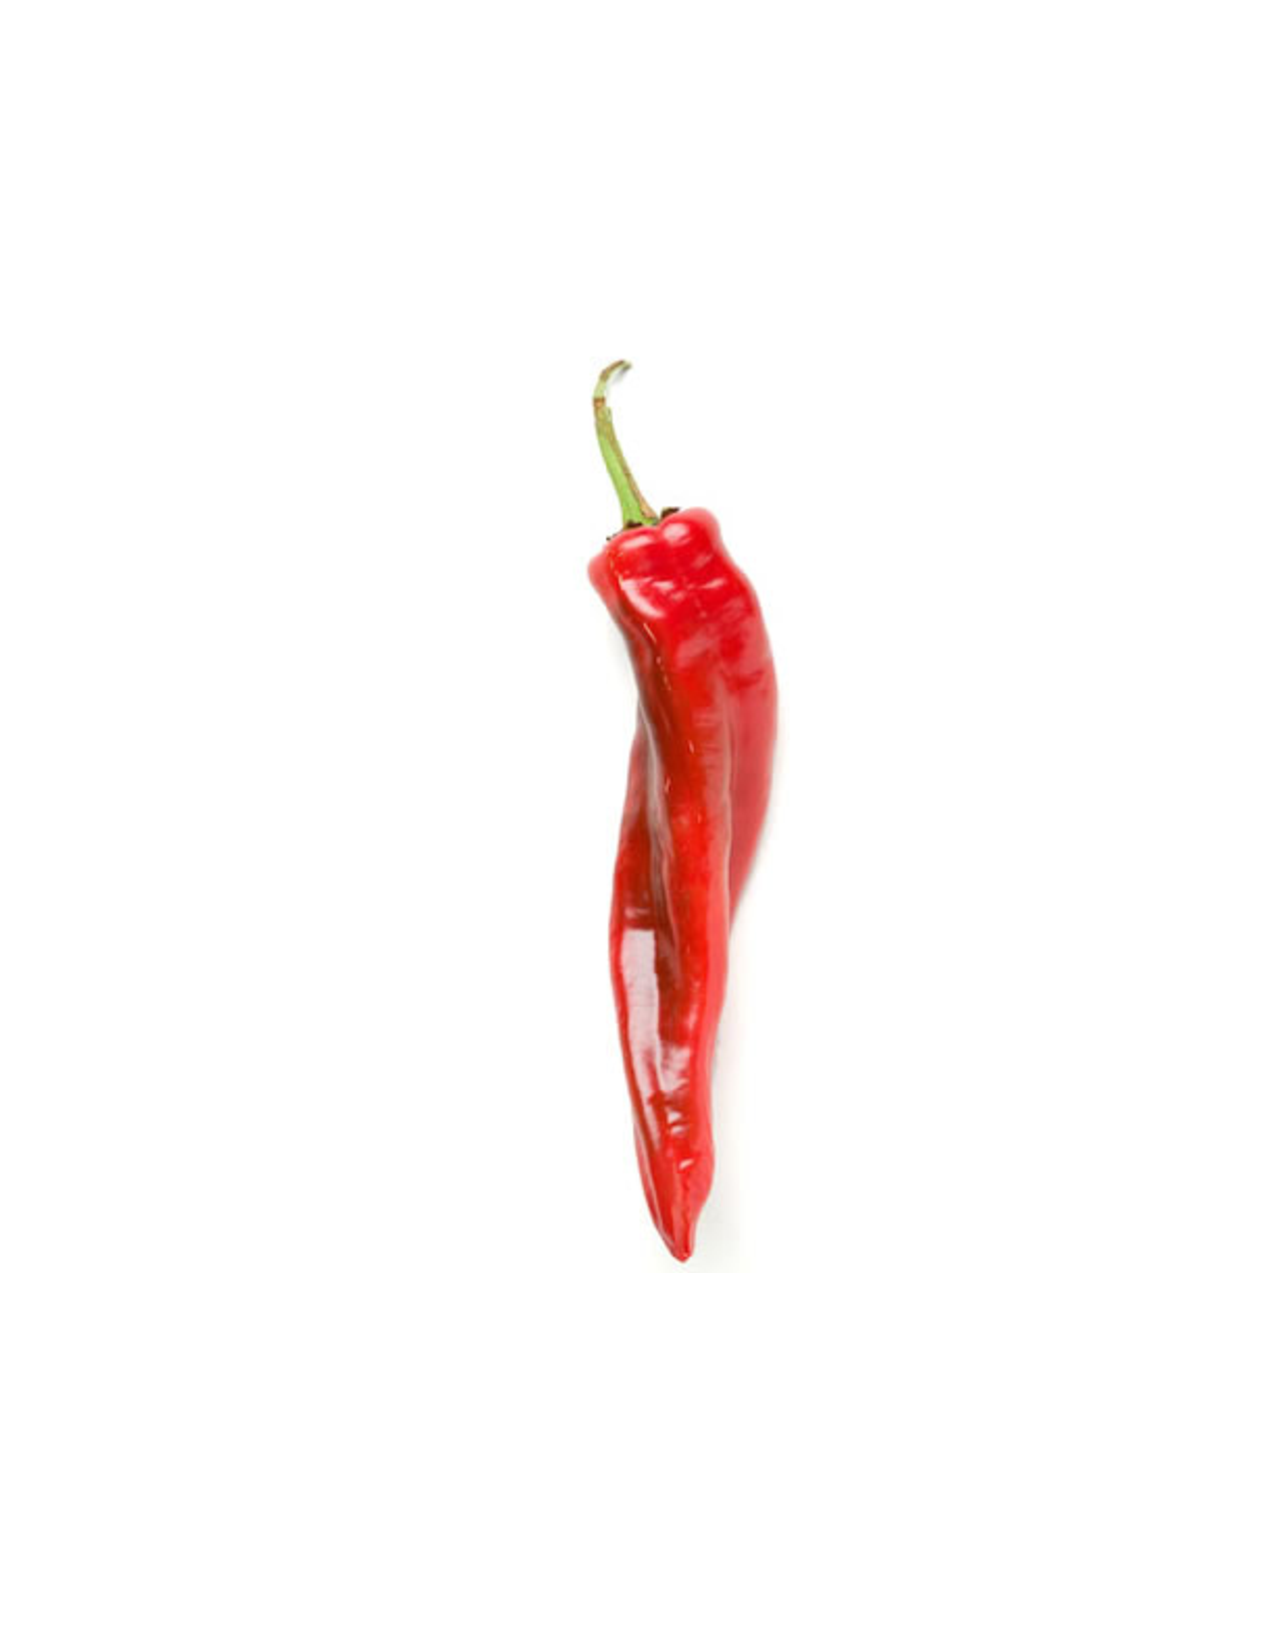
\includegraphics{figures/chili.pdf}}}
\newcommand{\chchili}{{\chili\chili}}
\newcommand{\chchchili}{{\chchili\chili}}

% The units package provides nice, non-stacked fractions and better spacing
% for units.
\usepackage{units}

% The fancyvrb package lets us customize the formatting of verbatim
% environments.  We use a slightly smaller font.
\usepackage{fancyvrb}
\fvset{fontsize=\normalsize}

% Small sections of multiple columns
\usepackage{multicol}

\hypersetup{
urlcolor=blue,
colorlinks=true
}
\usepackage[noline, procnumbered, linesnumberedhidden, boxed]{algorithm2e}

\newcommand{\openepigraph}[2]{ % This block sets up a command for printing an epigraph with 2 arguments - the quote and the author
\begin{fullwidth}
\sffamily\large
\begin{doublespace}
\noindent\allcaps{#1}\\ % The quote
\noindent\allcaps{#2} % The author
\end{doublespace}
\end{fullwidth}
}

\newcommand{\figref}[1]{Figure~\ref{#1}}
\renewcommand{\thefigure}{\arabic{figure}}

\newenvironment{callout}[1]{
\[
  \left[
      \begin{tabular}{@{\quad}m{.05\textwidth}@{\qquad}m{.75\textwidth}@{\quad}}
        \scalebox{1.5}{#1} & 
          \raggedright%
}
{
      \end{tabular}
    \right]
\]
}

\newcommand{\blankpage}{\newpage\hbox{}\thispagestyle{empty}\newpage} % Command to insert a blank page

\usepackage{makeidx} % Used to generate the index
\makeindex % Generate the index which is printed at the end of the document

\renewcommand{\maketitlepage}[0]{%
  \cleardoublepage%
  {%
  \sffamily%
  \begin{fullwidth}%
  ~
  \vspace{11.5pc}%
  \fontsize{36}{40}\selectfont\par\noindent\textcolor{darkgray}{\allcaps{\thanklesstitle}}%
  
\scalebox{.2}{
\includegraphics{figures/msan-logo}}
  \vspace{11.5pc}%
  \fontsize{12}{18}\selectfont\par\indent\textcolor{darkgray}{\allcaps{\thanklessauthor}\\
\indent{\tt parrt@cs.usfca.edu}\\
\href{http://parrt.cs.usfca.edu}{http://parrt.cs.usfca.edu}}%
  \vspace{11.5pc}%
  \fontsize{14}{16}\selectfont\par\noindent\allcaps{\thanklesspublisher}%
  \end{fullwidth}%
  }
  \thispagestyle{empty}%
  \clearpage%
}

\titlecontents{part}% FIXME
    [0em] % distance from left margin
    {\vspace{1.5\baselineskip}\begin{fullwidth}\LARGE\rmfamily\itshape} % above (global formatting of entry)
    {\contentslabel{2em}} % before w/label (label = ``II'')
    {} % before w/o label
    {\rmfamily\upshape\qquad\thecontentspage} % filler + page (leaders and page num)
    [\end{fullwidth}] % after

  \titlecontents{chapter}%
    [0em] % distance from left margin
    {\vspace{1.5\baselineskip}\begin{fullwidth}\Large\rmfamily\itshape} % above (global formatting of entry)
    {\hspace*{0em}\contentslabel{2em}} % before w/label (label = ``2'')
    {\hspace*{4em}} % before w/o label
    {\rmfamily\upshape\qquad\thecontentspage} % filler + page (leaders and page num)
    [\end{fullwidth}] % after

\titlespacing*{\chapter}{0pt}{0pt}{30pt}
\titlespacing*{\section}{0pt}{3.5ex plus 1ex minus .2ex}{2.3ex plus .2ex}
\titlespacing*{\subsection}{0pt}{3.25ex plus 1ex minus .2ex}{1.5ex plus.2ex}

\newcount\tmpnum
\def\tallymarks#1{\leavevmode \lower1bp\vbox to9bp{}%
   \tmpnum=#1
   \loop \ifnum\tmpnum<5 \kern1bp \tallynum\tmpnum \else \tallyV \fi
         \advance\tmpnum by-5
         \ifnum\tmpnum>0 \repeat
}
\def\tallynum#1{\bgroup\tmpnum=#1\relax
   \loop \ifnum\tmpnum>0
         \kern1bp \tallyI \kern1bp
         \advance\tmpnum by-1
         \repeat
   \egroup
}
\def\tallyI{\pdfliteral{q .5 w 0 -1 m 0 8 l S Q}}
\def\tallyV{\kern1bp\pdfliteral{q .5 w -1 0 m 9 7 l S Q}\tallynum4\kern1bp }



\begin{document}


\chapter{Representing Data}

\setcounter{problem}{1}

\section{Digitizing our world}

\begin{fullwidth}

Everything in the computer is stored as a number. This includes numbers of course as well as letters, audio files, movie files, etc.

\subsection{Unary}

``{\em One if by Land Two if by Sea}'' --Paul Revere

A single symbol or digit: 1.  It's the way we count with tick marks in groups of 5. \tallymarks{1}, \tallymarks{2}, \tallymarks{3}, \tallymarks{4}, \tallymarks{5}

\begin{center}
\begin{tabular}{|ccc|c|}
\hline
\multicolumn{3}{|c|}{Unary digits} & Value\\
\hline
&       &    & 0\\
&       & 1 & 1\\
& 1    & 1 & 2\\
1 & 1 & 1 & 3\\
\hline
\end{tabular}
\end{center}

\subsection{Binary}

Numbers are encoded in the machine using binary, 0 or 1 which corresponds to usually 0 and +5 Volts in the hardware. The fundamental element within a computer is a switch that can be either on or off just like a lightbulb. If I have one lightbulb, I can have two states: on or off, 0 or 1, lo or hi, whatever you want to call it. 

Q. If I have two lightbulbs, how many states can I have? 4

\begin{center}
\begin{tabular}{|cc|c|}
\hline
\multicolumn{2}{|c|}{Binary digits} & Value\\
\hline
0 & 0 & 0\\
0 & 1 & 1\\
1 & 0 & 2\\
1 & 1 & 3\\
\hline
\end{tabular}
\end{center}

What about three? $2^3 = 8$:

\begin{center}
\begin{tabular}{|ccc|c|c|}
\hline
\multicolumn{3}{|c|}{Binary digits} & Value & Count \\
\hline
0 & 0 & 0 & 0 & 1\\
0 & 0 & 1 & 1 & 2\\
0 & 1 & 0 & 2 & 3\\
0 & 1 & 1 & 3 & 4\\
1 & 0 & 0 & 4 & 5\\
1 & 0 & 1 & 5 & 6\\
1 & 1 & 0 & 6 & 7\\
1 & 1 & 1 & 7 & 8\\
\hline
\end{tabular}
\end{center}

These are two and three bit numbers, which indicates their maximum value.

A {\bf byte} is 8 bits. $2^8 = 256$ states or values 0..255.  A {\bf word} is typically the size of the microprocessor's registers. These days that will be 64 bits.

Binary numbers get long pretty quickly: {\tt 1010011010} binary is 666 decimal.

\subsection{Characters}

Everything is a number, so how to represent letters? (For now we we'll stick with the American character set). We assign a unique number to each letter:

\scalebox{.75}{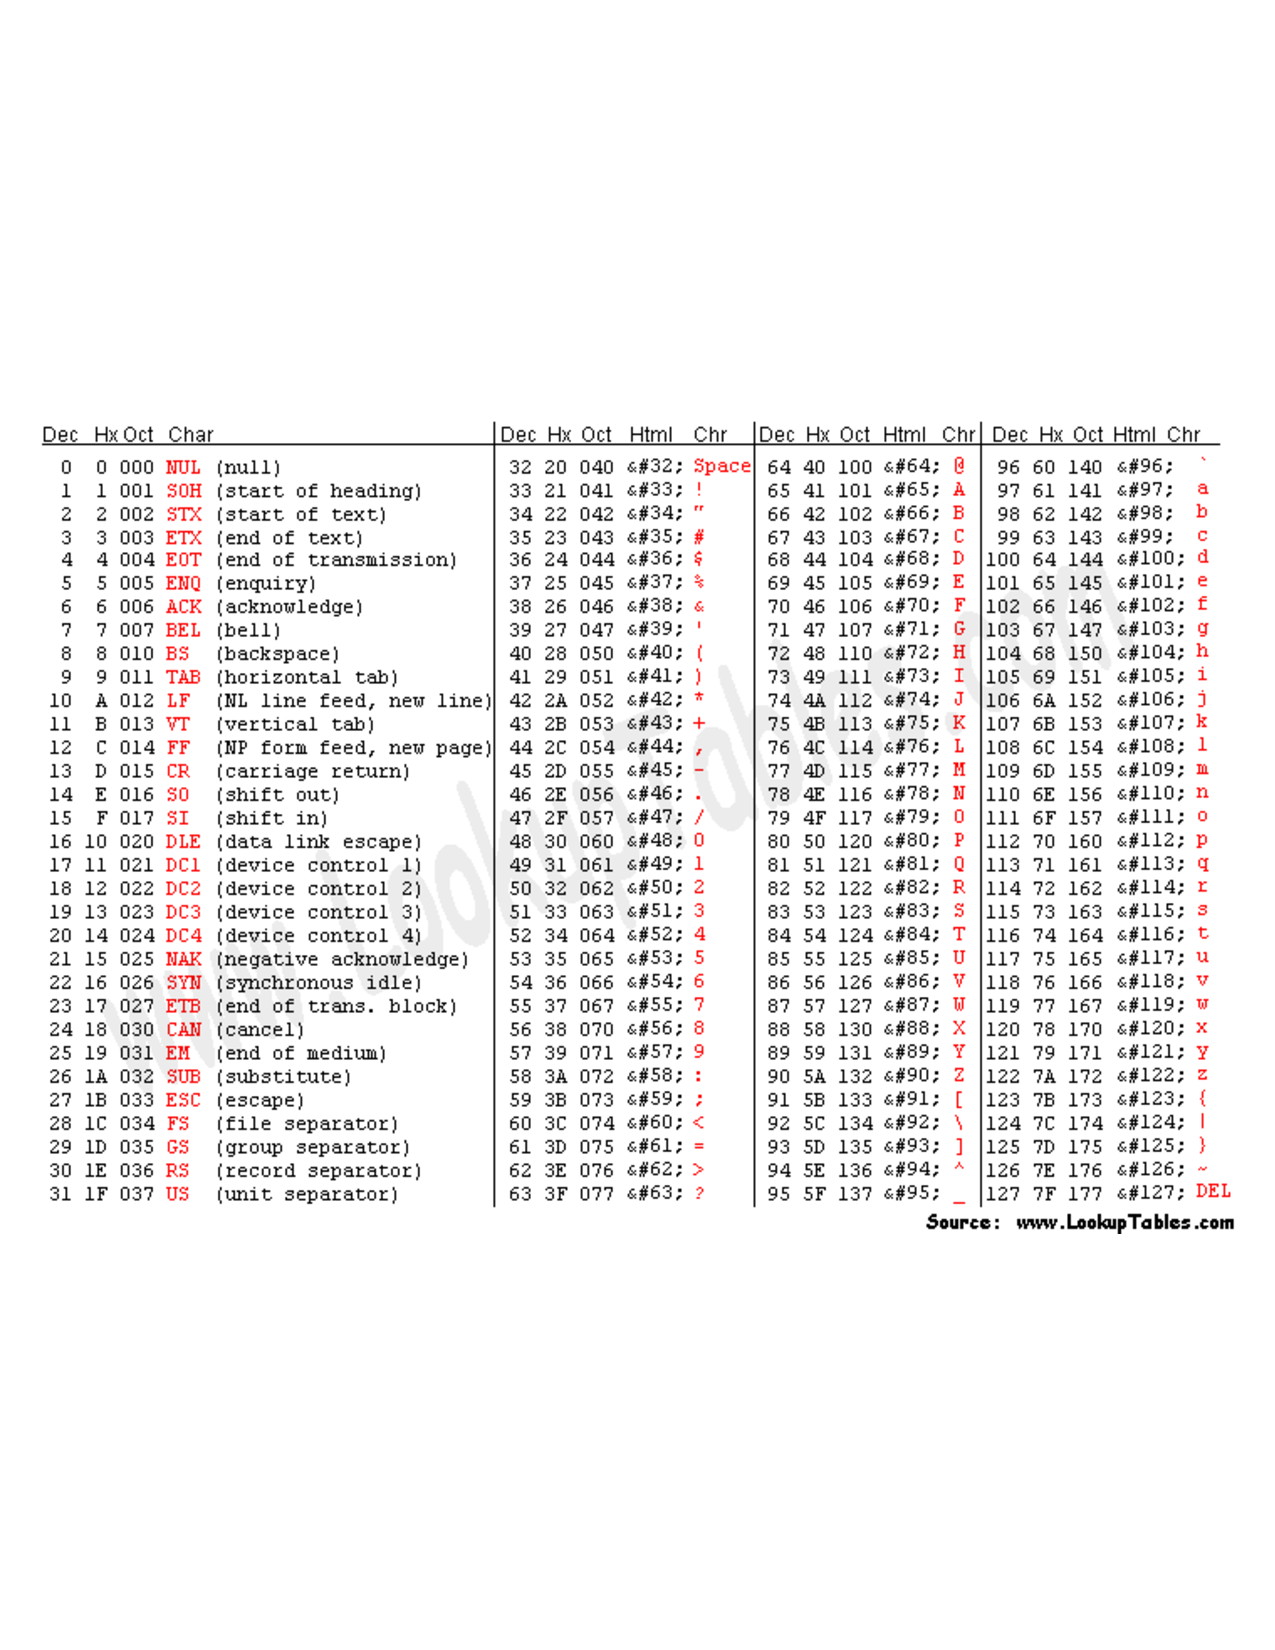
\includegraphics{figures/asciifull}}

You can think of this is kind of an encryption. Instead of saying ``Hi'' you might say ``73 105.''
 
There are multiple standards but the clear winner is \href{http://www.asciitable.com/}{ASCII}. In the old days there was also \href{http://www.lookuptables.com/ebcdic_scancodes.php}{EBCDIC}.

As we will see shortly, a phrase or sentence or word is just a sequence of characters hence a sequence of numbers stored in the machine.

\begin{alltt}\small
$ cat sentence.txt 
As we will see shortly, a phrase or sentence or word is just a sequence
of characters hence a sequence of numbers stored in the machine.
$ od -b sentence.txt
0000000   101 163 040 167 145 040 167 151 154 154 040 163 145 145 040 163
0000020   150 157 162 164 154 171 054 040 141 040 160 150 162 141 163 145
0000040   040 157 162 040 163 145 156 164 145 156 143 145 040 157 162 040
0000060   167 157 162 144 040 151 163 040 152 165 163 164 040 141 040 163
0000100   145 161 165 145 156 143 145 012 157 146 040 143 150 141 162 141
0000120   143 164 145 162 163 040 150 145 156 143 145 040 141 040 163 145
0000140   161 165 145 156 143 145 040 157 146 040 156 165 155 142 145 162
0000160   163 040 163 164 157 162 145 144 040 151 156 040 164 150 145 040
0000200   155 141 143 150 151 156 145 056 012                            
0000211
$ od -c -b sentence.txt
0000000   101 163 040 167 145 040 167 151 154 154 040 163 145 145 040 163
           A   s       w   e       w   i   l   l       s   e   e       s
0000020   150 157 162 164 154 171 054 040 141 040 160 150 162 141 163 145
           h   o   r   t   l   y   ,       a       p   h   r   a   s   e
0000040   040 157 162 040 163 145 156 164 145 156 143 145 040 157 162 040
               o   r       s   e   n   t   e   n   c   e       o   r    
0000060   167 157 162 144 040 151 163 040 152 165 163 164 040 141 040 163
           w   o   r   d       i   s       j   u   s   t       a       s
0000100   145 161 165 145 156 143 145 012 157 146 040 143 150 141 162 141
           e   q   u   e   n   c   e  \textbackslash{n}   o   f       c   h   a   r   a
0000120   143 164 145 162 163 040 150 145 156 143 145 040 141 040 163 145
           c   t   e   r   s       h   e   n   c   e       a       s   e
0000140   161 165 145 156 143 145 040 157 146 040 156 165 155 142 145 162
           q   u   e   n   c   e       o   f       n   u   m   b   e   r
0000160   163 040 163 164 157 162 145 144 040 151 156 040 164 150 145 040
           s       s   t   o   r   e   d       i   n       t   h   e    
0000200   155 141 143 150 151 156 145 056 012                            
           m   a   c   h   i   n   e   .  \textbackslash{n}
0000211
\end{alltt}

\subsection{Images}

Images are stored as numbers also.

For black and white images, we can use a single bit to represent a black-and-white  pixel where zero means off and one means on:

\scalebox{.15}{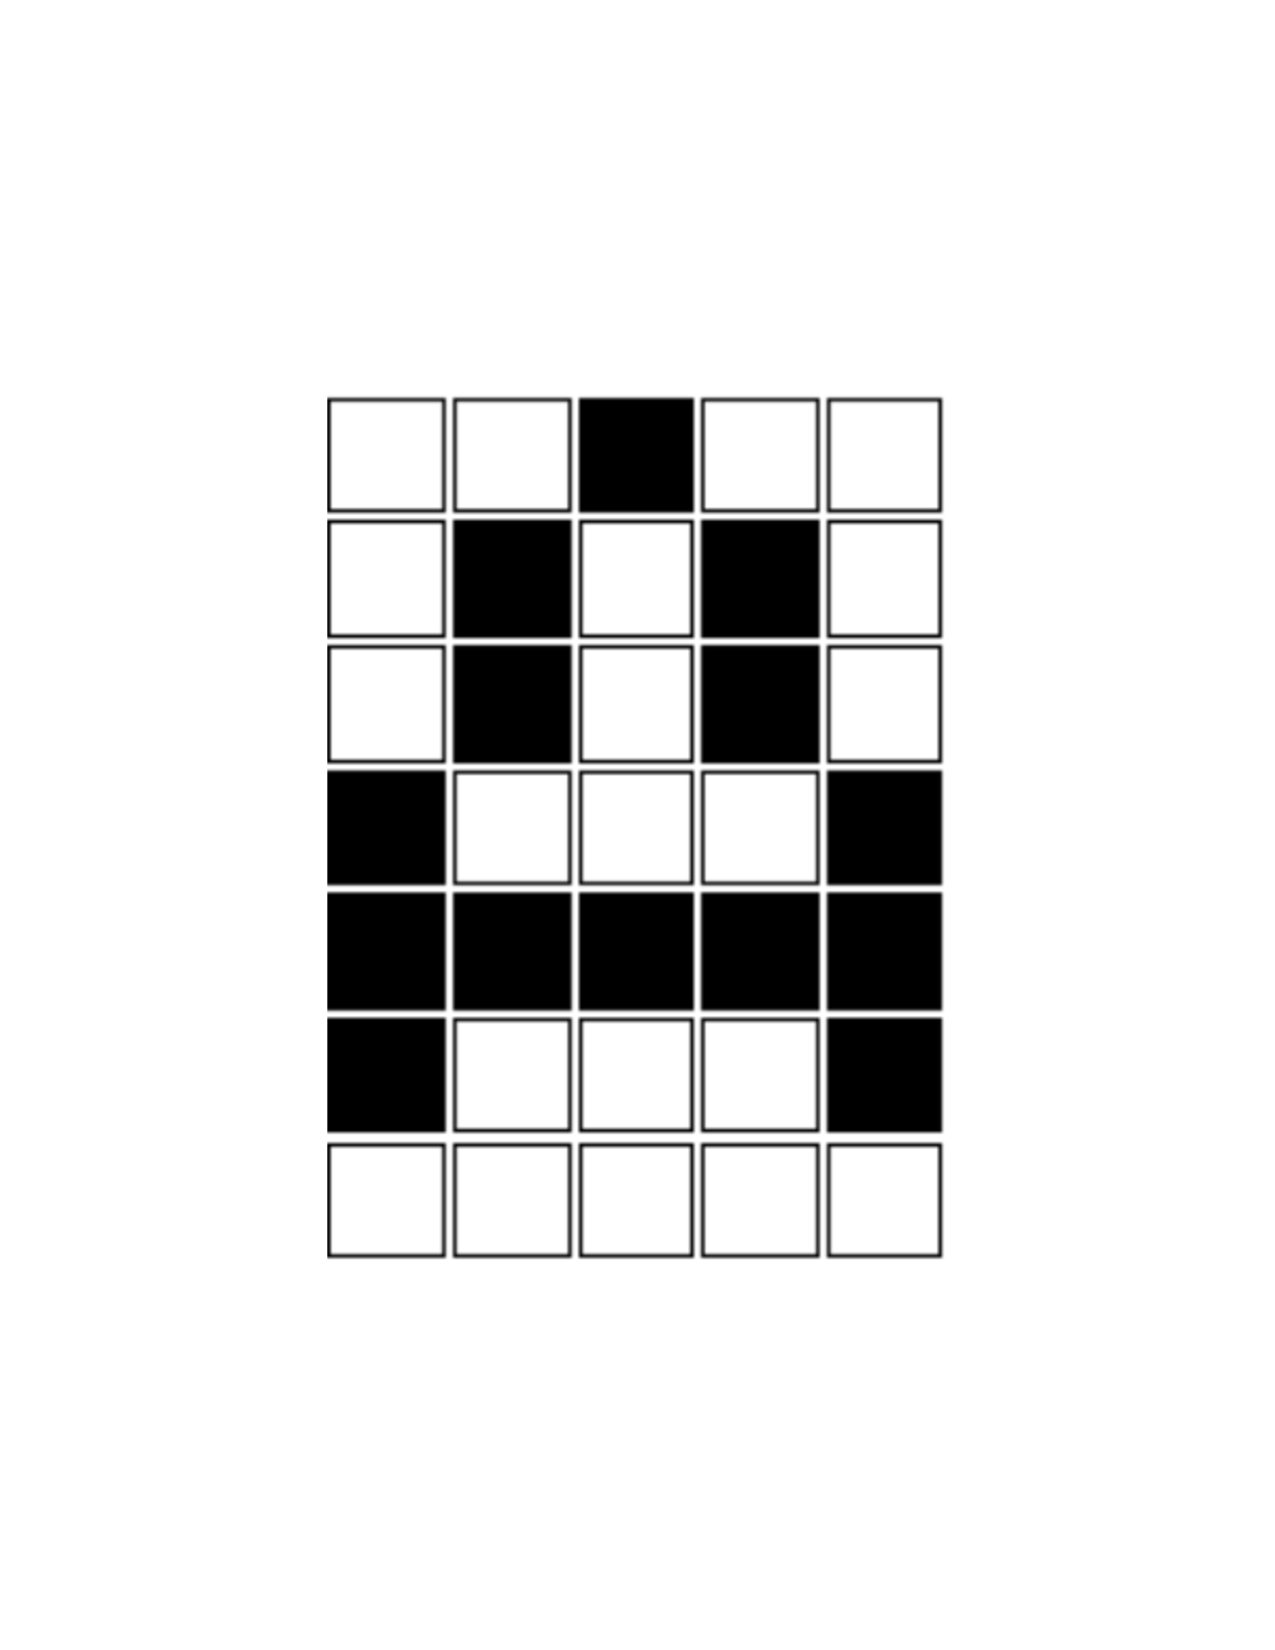
\includegraphics{figures/a-image}}

\noindent The bit sequence is:

{\tt 00100 01010 01010 10001 11111 10001 00000}

\noindent If you stack vertically, you can see the image sort of:

{\tt 00100\\
     01010 \\
     01010 \\
     10001 \\
     11111 \\
     10001 \\
     00000}

Each pixel on the screen is typically represented by three numbers, though: (red, green, blue) RGB values. For example:

white: 255 255 255  (yes they are one byte each) \\
black: 0 0 0\\
blue: 0 0 255 (blue is saturated)\\
Yellow is a mix of red and green: 255 255 0


\subsection{Audio}

Audio files that you listen to are also represented as just a sequence of numbers where each number represents the amplitude of the signal at discrete locations and time. From Wikipedia page on \href{https://en.wikipedia.org/wiki/Digital_audio}{Digital audio}:

\scalebox{.35}{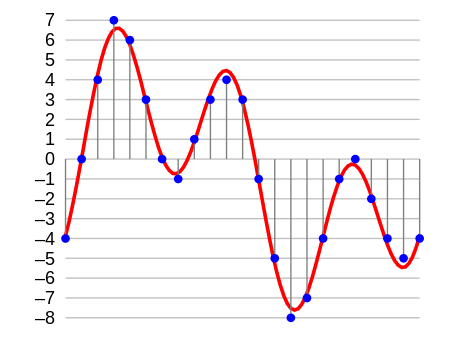
\includegraphics{figures/waveform-quant.png}}

Here is a partial waveform of Prince's ``Kiss'' song:

\scalebox{.35}{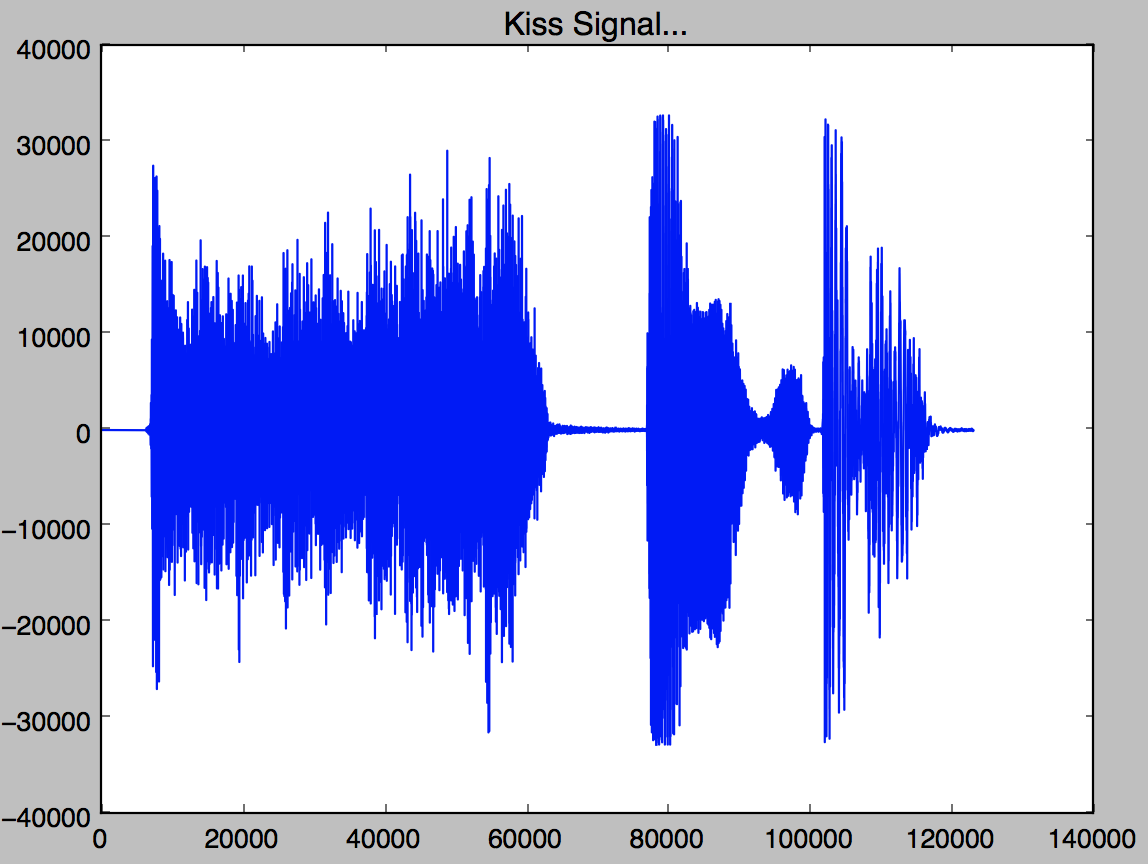
\includegraphics{figures/kiss-signal.png}}

\noindent I loaded via a sample program in {\tt notes/code/plotaiff.py}:

\begin{alltt}
$ cd notes/code
$ python plotaiff.py ../../data/Kiss.aiff 
$ open ../../data/Kiss.aiff # play the audio
\end{alltt}

\noindent ({\em BTW, that ``{\tt ..}'' means jump up a directory})

\noindent Q. What to those values represent?

\noindent Q. What happens if you scale each value?

\begin{alltt}
$ python scaleaiff.py ../data/Kiss.aiff /tmp/scaled-kiss.aiff
$ open /tmp/scaled-kiss.aiff
\end{alltt}

\noindent Sample code: \href{https://github.com/parrt/msan501/blob/master/notes/code/plotaiff.py}{\textcolor{blue}{plotaiff.py}}, \href{https://github.com/parrt/msan501/blob/master/notes/code/scaleaiff.py}{\textcolor{blue}{scaleaiff.py}}.

\subsection{Entropy}

It could be a good time to mention the term \href{https://en.wikipedia.org/wiki/Entropy_\%28information_theory\%29}{\textcolor{blue}{entropy}}, which is a measure of the chaos or disorder of a model or system. In the real world, systems always tend towards increased entropy. For example, the state of my kitchen approaches maximum entropy two weeks after the maid has cleaned up. You will see entropy again when you look at algorithms to construct random forests. Entropy in information theory describes how much information is in a signal.

Q.  Does it take more bits or fewer bits to store random noise compared to, for example, a pure tone at a particular frequency?

If you need to store a random variable that can take $n$ values with equal probability, you need $log_2(n)$ bits to represent that variable/number. On the other hand, if we know for sure that the random variable is always, say, 9345 or 0 then it only takes a single bit to represent that random variable (9345 is present or not).
 
\section{Python's atomic elements}

There are a few basic or atomic elements in Python and each kind of element knows not only its value but also its type. It's very important to learn the difference between value and type. Python does not expect you to specify the type of a variable, but of course it runtime it has an exact type. As a programmer we must be aware of these types so that we don't try to divide two strings, for example.

\subsection{Integers}

These are just numbers that were used for counting; whole numbers like -9, 0, 3, 1023023823. What are the types/sizes?

\begin{pyconsole}[b]
type(1000000000000000000)
type(10000000000000000000)
\end{pyconsole}

How many bits to store?

\begin{pyconsole}[b]
import math
math.log(1000000000000000000, 2)
math.log(10000000000000000000, 2)
\end{pyconsole}

You can make these things as big as you like:
 
\begin{pyconsole}[a]
type(323241321234123412348123091324)
\end{pyconsole}

But if they are smaller they go into a different type. {\tt type} is just another function call that asks the type of something.

\begin{pyconsole}[b]
type(3232)
\end{pyconsole}


\subsection{Real numbers}
 
Real numbers, not whole numbers, are of finite precision but can hold some very large and very small numbers.

\begin{pyconsole}[c]
3.14159
0.000000000001
23e100
\end{pyconsole}

The {\tt e} stuff is the scientific notation and represents the exponent, not the mathematical constant $e$. We call these {\em floating-point numbers}.

The \href{https://docs.python.org/2/tutorial/floatingpoint.html}{\textcolor{blue}{Python tutorial on floating-point numbers}} is something you should look at to learn more about floating-point numbers. The fact that they have finite precision, so-called ``double precision,'' means you can get some odd results:

\begin{pyconsole}[z]
0.1 + 0.2
\end{pyconsole}

\noindent This is because 0.1 is actually represented as 0.00011001100110011..., a repeating fraction.  It has no nice representation in binary fractions, but numbers like 0.125 = 1/8 do: 0.001 in binary = $\frac{0}{2^1}+\frac{0}{2^2}+\frac{1}{2^3}$.

If you need floating-point numbers that trade precision for efficiency, use the \href{https://docs.python.org/2/library/decimal.html#module-decimal}{\textcolor{blue}{decimal}} module:

\begin{pyconsole}[z2]
from decimal import Decimal
Decimal(1)/Decimal(10) + Decimal(2)/Decimal(10)
\end{pyconsole}

One last thing on Floating-point numbers. {\em Be aware that subtraction can destroy precision}. It is considered an ill conditioned operation because subtracting two numbers that are almost equal can give you very imprecise answers.

\subsection{Boolean values}

A Boolean value is either true or false, but Python also allows a number of other things to represent true and false such as 1 can be true and 0 can be false.

\begin{pyconsole}[d]
True
False
bool(1)
bool(0)
bool(36)
bool("hi")
\end{pyconsole}

All of the comparison and logical operators yield Boolean types:

\begin{pyconsole}[d]
1 < 10
3.4 >= 10+0.2
"cat" < "dog"
1 < 10 and "a"<"b"
False or True
\end{pyconsole}

\subsection{Strings}

Single, double, or triple quotes. 0 or more characters in between delimiters. We call these literals or hardcoded values.

\begin{pyconsole}[e]
'a'  # a single character string is sometimes called a character
'hi'
"hi"
"""hi"""
\end{pyconsole}

When you need to actually include quotes of some kind in the string, then you surround it with different quotes like {\tt "Bob's house"}.

\subsection{Special characters}

{\tt \textbackslash n}  is the newline character, {\tt \textbackslash t}  is the tab character


\begin{pyconsole}[f]
print "Cars:\n\tBMW\n\tAudi"
\end{pyconsole}

which is like doing:
 
\begin{pyconsole}[g]
print "Cars:"
print "\tBMW"
print "\tAudi"
\end{pyconsole}

or

\begin{pyconsole}[h]
print "Cars:"
print "	BMW"
print "	Audi"
\end{pyconsole}


\subsection{Conversions}

We can convert between numbers

\begin{pyconsole}[i]
float(3)
int(3.14159)
\end{pyconsole}

\noindent and numbers and characters

\begin{pyconsole}[j]
chr(100)
chr(105)
ord('H')
str(234)
\end{pyconsole}

What the types of operands.

\begin{pyconsole}[j]
"hi" + 501
"hi" + str(501)   # convert number to string then add
2 / 3
2 / float(3)
2 / 3.0
10 == 10
10 == "10"
\end{pyconsole}

\end{fullwidth}

\end{document}